\chapter{Contact-aware Multibody Dynamics}
\label{ch:contact_aware_dynamics}

In the first part of this thesis contributions, we proposed a general framework for creating robotic environments and, with it, introduced a scheme for training a policy for generating push-recovery control signals balancing the iCub humanoid robot in the presence of external disturbances.
The simulations were performed using the general-purpose Gazebo Sim, which provides a rich ecosystem supporting many types of robots, sensors, physics engines, and rendering capabilities.
However, the benefits of exploiting general-purpose solutions often introduce a trade-off with the achievable performance.
As we have experienced with the push-recovery policy presented in Chapter~\ref{ch:learning_from_scratch}, a single iteration of policy training could last multiple days, resulting in a long tuning process that could limit the search space.
The bottleneck of the training pipeline are the computations performed by the rigid-body simulator, limiting the rate at which new trajectories can be sampled.

In the continuation of this thesis, we attempt to reply to the question: \textit{"How can we optimise sampling performance of synthetic data?"}.
In this chapter, we derive the state-space representation of a floating-base multibody system interacting with a known ground surface.
Assuming the knowledge of the terrain height at any point in space and the smoothness of the terrain surface, this formulation of the dynamics enables calculating the robot's trajectory using a plain numerical integration scheme, regardless of the contact state.
To this end, we introduce a continuous soft-contacts model for resolving points-surface collisions supporting both static (sticking) and dynamic (slipping) contacts.
Each contact point's dynamics state is structured such that it can be included in the state-space representation and integrated with the robot's dynamics.
The resulting representation will be used, in the next chapter, as a base for a novel physics engine targeted to exploit modern hardware accelerators for maximising trajectory sampling.

\section{Notation}

\subsection{Frame kinematics with quaternions}
\label{sec:frame_kinematics_quaternion}

In Chapter~\ref{ch:robot_modelling}, we introduced the homogeneous transformation $\homo[A]_B \in \SE(3)$ to describe the pose of a frame (corresponding also to a rigid body).
An alternative representation of the $\SE(3)$ group is the tuple $(\pos[A]_B, {}^A \bar{q}_B)$, where $\pos[A]_B \in \realn^3$ is the \emph{position vector} and ${}^A \bar{q}_B$ a \emph{unit quaternion}.
A generic quaternion can be defined as follows:
%
\begin{equation*}
    q \in \mathbb{H} := \left\{ q_w + \hat{i} q_x + \hat{j} q_y + \hat{k} q_z \;:\;\; q_w, q_x, q_y, q_z \in \realn \right\}
    ,
\end{equation*}
%
where $\Re(q) = q_w$ is the \emph{real} part of the quaternion and $\Imag(q) = \hat{i} q_x + \hat{j} q_y + \hat{k} q_z$ is the \emph{imaginary} part.
Elements of $\SO(3)$ describing frame rotations can be described by \emph{unit quaternions}:
%
\begin{equation*}
    \bar{q} \in \Spin(3) := \left\{ q \in \mathbb{H} \;:\; |q| = 1 \right\}
    .
\end{equation*}
%
A quaternion could be also described with a real vector of its coefficients:
%
\begin{equation*}
    \quat = (w, \mathbf{r}) \in \realn^4
    ,
\end{equation*}
%
where $w = q_w \in \realn$ and $\mathbf{r} = (q_x, q_y, q_z) \in \realn^3$.
In this chapter, we mainly use this last representation since it has a direct relation with the practical usage in algorithms design.
The pose of a generic frame can therefore be described by a vector $(\pos[A]_B, \quat[A]_B) \in \realn^7$.
%
For what regards the frame velocity, we can keep using any of the 6D vectors introduced in Section~\ref{sec:frame_velocities}, \ie $\velsix_{A,B} = (\vellin_{A,B}, \velang_{A,B}) \in \realn^6$.

\subsection{Frame pose derivative and 6D velocity with quaternions}

When the orientation of a frame is expressed with a quaternion, it's worth introducing the relation between the derivative of the pose $(\posd[A]_B, \quatd[A]_B) \in \realn^7$ and the 6D velocity $\velsix_{A,B} \in \realn^6$.
In fact, particularly in this case with the quaternion, it's clear that the two cannot be related by a simple numerical differentiation since they also have different dimensions.
The following relations hold:
%
\begin{equation}
    \label{eq:pose_dot_with_quaternion}
    \begin{cases}
        \posd[A]_B = \vellin[{A[B]}]_{A,B} \\
        \quatd[A]_B = \frac{1}{2} S(\velang[B]_{A,B}) \quat[A]_B
    \end{cases}
    ,
\end{equation}
%
where we notice that the derivative of the position is the linear part of the mixed velocity defined in Equation~\eqref{eq:mixed_velocity} (denoted as $\orid[A]_B$), and defined the derivative of the quaternion~\parencite{sola_quaternion_2017} by introducing the following matrix:
%
\begin{equation*}
    \operatorname{S}(\velang) =
    \begin{bmatrix}
        0 & -\velang^\top \\ \velang & -\velang^\wedge
    \end{bmatrix}
    .
\end{equation*}

The relations of Equation~\eqref{eq:pose_dot_with_quaternion} can be used for integrating numerically the frame pose, using one of the schemes that will be introduced in Section~\ref{sec:integrators}.
The quaternion $\quat$, in this setting, has to be treated with care, because only unit quaternions can describe rotations.

Numerical integration schemes do not enforce this property is maintained along the trajectory, and numeric approximations could lead to unwanted instabilities.
This problem can be either solved or mitigated by different types of solutions.
The most straightforward solution is normalising the quaternion after each integration step.
Alternatively, a correction term orthogonal to the quaternion dynamics of the following form can be introduced:
%
\begin{equation*}
    \quatd = \frac{1}{2} \operatorname{S}\left( \rot[B]_W \velang[W]_{W,B} \right) \quat + \frac{1}{2} K_{\quat} \quat \left( \norm{\quat}^{-1} - 1 \right)
    ,
\end{equation*}
%
that corresponds to a Baumgarte stabilization on $\SO(3)$~\parencite{gros_baumgarte_2015}, where $K_{\quat} \in \realn$ is the correction coefficient.
This stabilization term progressively projects the quaternion towards a unity quaternion, restoring the norm in case of drifting.
In the continuation of this thesis, we do not explicitly include any correction, considering its choice an implementation detail.

\begin{remark*}[Geometric integration of quaternions]
%
Quaternions, like other representations of elements of $\SO(3)$, have strong geometrical properties based on the underlying symmetries.
These properties can be exploited to obtain more rigorous integration schemes performed directly on the manifold~\parencite{andrle_geometric_2013}.
The quaternion relation of Equation~\eqref{eq:pose_dot_with_quaternion} can be seen as a differential equation in $\quat[A]_B$.
By exploiting properties of the matrix exponential together with quaternion properties, it can be shown~\parencite{andrle_geometric_2013, sola_quaternion_2017, sola_micro_2020} that the following relation implements a zero-\emph{th} order integration:
%
\begin{align*}
    \quat_{t_{k+1}} = \quat_{t_k} \otimes \left( \norm{\velang}\cos(\velang \Delta t / 2), \frac{}{} \sin(\velang \Delta t / 2) \right)
\end{align*}
%
where $\otimes$ denotes the quaternion multiplication, and $\velang$ is assumed constant within the integration interval $[t_k, t_{k+1}]$.

While both integration approaches are valid options --albeit showing different numerical stability \parencite{andrle_geometric_2013}--, we develop the theory of this chapter using the numerical derivative.
This choice allows treating the entire state of a multibody system, including the base quantities, as a vector in $\realn^n$, simplifying the equations of this chapter.
If needed, practical implementations of the presented results could adopt the geometrical integration if better numerical stability is required, paying the price to treat the base orientation separately.
%
\end{remark*}

\subsection{Multibody dynamics}

The \acp{EoM} of a floating-base multibody system have been previously introduced in Section~\ref{sec:multibody_dynamics} in the following form:
%
\begin{equation*}
    M(\Qu) \Nud + C(\Qu, \Nu) \Nu + g(\Qu) = B \Torques + \sum_{\mathcal{L}} J_{L}^\top(\Qu) \forcesix_L^{ext}
    ,
\end{equation*}
%
where $\Qu$ is the generalised position and $\Nu$ is the generalised velocity already introduced in Equation~\eqref{eq:floating_base_velocity}.
%
If a quaternion $\quat[W]_B$ is used to model the orientation of the base frame $B$, as described in Section~\ref{sec:frame_kinematics_quaternion}, we can expand the generalised position and velocity as follows:
%
\begin{align}
    \label{eq:qu_nu_quaternion}
    \mathbf{q} &= \left( \pos[W]_B,  \quat[W]_B, \mathbf{s} \right) \in \mathbb{R}^{n+7} \\
    \boldsymbol{\nu} &= \Nu[W] = \left( \vellin[W]_{W,B}, \velang[W]_{W,B}, \dot{\mathbf{s}} \right) \in \mathbb{R}^{n+6}
    ,
\end{align}
%
where we chose the inertial-fixed representation of the base velocity, introduced in Section~\ref{sec:right_trivialized_velocity}, just for practical reasons.

When the explicit decomposition of the Coriolis and gravitational terms is not required, we combine their effects into the following vector of \emph{bias forces}:
%
\begin{equation*}
    h(\Qu, \Nu) = C(\Qu, \Nu) \Nu + g(\Qu) \in \realn^{6+n}
    .
\end{equation*}

We can compact the Lagrangian formulation of the system's dynamics even more by updating the terms related to the external 6D forces.
We assume, for each link $L \in \mathcal{L}$, that an external 6D force $\forcesix^{ext}_L$ always exists but is zero if the link has no interaction with the environment.
If we stack the Jacobians and the 6D forces of all links in the following new matrices:
%
\begin{align*}
    J_\mathcal{L}(\Qu) = 
    \begin{bmatrix}
        J_0 \\
        J_1 \\
        \vdots \\
        J_{n_L - 1}
    \end{bmatrix} \in \mathbb{R}^{6 n_L \times 6+n},
    && 
    \forcesix^{ext}_\mathcal{L} = 
    \begin{bmatrix}
        \forcesix_0 \\
        \forcesix_1 \\
        \vdots \\
        \forcesix_{n_L - 1}
    \end{bmatrix} \in \mathbb{R}^{6 n_L}
    ,
\end{align*}
%
we can replace the sum with a more compact matrix product:
%
\begin{equation}
    \label{eq:eom_multibody_compact}
    M(\Qu) \Nud + h(\Qu, \Nu) = B \Torques + J_\mathcal{L}^\top(\Qu) \forcesix^{ext}_\mathcal{L}
    .
\end{equation}

\section{State-space Multibody Dynamics}

The \acp{EoM} of a multibody system of Equation~\eqref{eq:eom_multibody_compact} are expressed as non-linear \ac{ODE}.
Modern control theory studies the properties of these systems studied by operating on their \emph{state-space} representation~\parencite{friedland_control_2005}, which assumes the following general form:
%
\begin{equation}
\label{eq:state_space_representation}
\begin{cases}
    \mathbf{x}(t) &= f \left( t, \mathbf{x}(t), \mathbf{u}(t) \right) \\
    \mathbf{y}(t) &= g \left( t, \mathbf{x}(t), \mathbf{u}(t) \right)
\end{cases}
,
\end{equation}
%
where the first is the \emph{state equation} and the second is the \emph{output equation}.
The variable $\mathbf{x}$ is called \emph{state vector} and the variable $\mathbf{u}$ is called \emph{input vector}.
State-space models are particularly interesting for computing, starting from a given initial state $\mathbf{x}_0$, the future trajectory of an arbitrarily complex system, under the assumption of the complete knowledge of its dynamics $f(\cdot)$ and inputs $\mathbf{u}(t)$, if any.
In the most general case, even when closed-form solutions of Equation~\eqref{eq:state_space_representation} cannot be found, future trajectories can be computed through numerical integration~\parencite{cellier_continuous_2006}, as it will be described in Section~\ref{sec:integrators}.

In the case of a rigid multibody system, the \acp{EoM}~\eqref{eq:eom_multibody_compact} can be expressed in state-space representation by introducing the following state and input vectors:
%
\begin{align}
    \label{eq:input_and_state_vectors}
    \mathbf{x}(t) =
    \begin{bmatrix}
        \Qu \\ \Nu
    \end{bmatrix}
    \in \mathbb{R}^{2n+13},
    &&
    \mathbf{u}(t) =
    \begin{bmatrix}
        \Torques \\ \forcesix^{ext}_\mathcal{L} 
    \end{bmatrix}
    \in \mathbb{R}^{n+6n_L}.
\end{align}
%
With these definitions, we can define the state equation of our system as:
%
\begin{equation*}
    \dot{\mathbf{x}}(t) =
    \begin{bmatrix}
        \dot{\mathbf{q}} \\ \dot{\boldsymbol{\nu}}
    \end{bmatrix} =
    f\left(\mathbf{x}(t), \mathbf{u}(t)\right)
    ,
\end{equation*}
%
where we still need to find the equations of $\Qud$ and $\Nud$.

The variable $\Nud \in \realn^{6+n}$ is the \emph{generalised acceleration} of the system.
Assuming the mass matrix $M(\Qu)$ non-singular, the dynamics of $\Nu$ can be extracted directly from the \acp{EoM}~\eqref{eq:eom_multibody_compact}.
As we will introduce in Chapter~\ref{ch:scaling_rigid_body_simulations}, the computation of $\Nud$ is also known as \emph{forward dynamics} of the multibody system, and the methodology that requires the inversion of the mass matrix is just one among the available methods, not necessarily the most computationally efficient.
In order to maintain a degree of generality, in this chapter we mark this computation with the $\operatorname{FD}(\cdot)$ function.

For what regards $\Qud$, we can simply extend the base quantities of Equation~\eqref{eq:pose_dot_with_quaternion} with the joint velocities $\dot{\mathbf{s}}$.
The advantage of using the numerical integration form of the quaternion should now be clear, since it enables its direct inclusion in the state vector.

The final form of the state-space representation can be found by combining all the previous elements:
%
\begin{equation}
    \label{equation:floatig_base_dynamics_state_space}
    \dot{\mathbf{x}}(t) =
    \begin{bmatrix}
        \Qud \\ \Nud
    \end{bmatrix} =
    \begin{bmatrix}
        \begin{pmatrix}
            \posd[W]_B \\
            \frac{1}{2} \operatorname{S}\left( \rot[B]_W \velang[W]_{W,B} \right) \quat[W]_B \\
            \dot{\mathbf{s}}
        \end{pmatrix}
        \\
        \operatorname{FD}(\mathcal{M}, \Qu, \Nu, \Torques, \forcesix_\mathcal{L}^{ext})
    \end{bmatrix} =
    f\left(\mathbf{x}(t), \mathbf{u}(t)\right)
    .
\end{equation}
%
Also in this case, it's worth noting that $\Qud \neq \Nu$, due to the nature of the angular variables of the base link. 

Computing the evolution of this system requires the knowledge of its inputs, represented by the joint torques $\Torques$ and the external forces $\forcesix_{\mathcal{L}}^{ext}$.
The external forces could either be known 6D forces supplied by the user, or unknown 6D forces resulting from the interaction with the environment:
%
\begin{equation}
    \label{eq:decomposition_external_forces}
    \forcesix_\mathcal{L}^{ext} = \forcesix_\mathcal{L}^{user} + \forcesix_\mathcal{L}^{contact}
\end{equation}
%
In the next section, we describe a methodology to compute the unknown forces exchanged with the environment by assuming that the floating-base model only interacts with the terrain $\forcesix_\mathcal{L}^{contact} := \forcesix_\mathcal{L}^{terrain}$, assumption compatible with our locomotion setting.
In a more general setting, $\forcesix_\mathcal{L}^{contact}$ should also include the forces exchanged between bodies, for example to simulate either self-collisions or interaction with other bodies part of the scene, particularly useful for robot manipulation.

\newpage
\section{Contact model}
\label{section:contact_model}

Detecting and handling contacts between bodies is one of the most challenging processes of a rigid-body simulation.
For simplicity, we assume that only contacts between points belonging to the model and a terrain surface can occur.
Considering our locomotion scenario, this assumption allows us to describe robots with collision shapes composed of a set of \emph{collidable points}.
This approach enables a unified logic for shapes ranging from simple boxes to complex meshes.
Note, however, that point-surface collisions do not provide expected results when a primitive shape like a box, modelled for example with its eight corner points, falls over the tip of a triangle-shaped terrain surface.
In this case, the collision detection should consider the box as a surface instead of a set of points.
If this use case is relevant, a possible workaround would be adding new collidable points on the box's surface, at a higher computational cost.
Despite this limitation, the point-surface model could suffice in many target scenarios.

\textcite{gilardi_literature_2002} distinguished two different approaches for impact and contact analysis: \emph{discrete} methods (also known as impulse-momentum) and \emph{continuous} methods.
They have shown that continuous methods are better suited for scenarios involving multiple contacts and bodies, allow for a better description of real systems, and simplify the inclusion of frictional effects.
The main drawback is the introduction of at least two parameters that need to be appropriately identified to match the real contact dynamics.
In robot learning, often this limitation is not particularly relevant since we can apply domain randomization over a realistic range of values.
Also, in our setting, a continuous contact model has the advantage of providing smooth gradients when used in an \ac{AD} context.

In the following sections, we first provide a description of the point-surface setting, introducing all the necessary elements for the contact model.
Then, we provide a more detailed analysis of continuous methods for \emph{collisions handling}, specifying how they can model both the \emph{normal} and the \emph{tangential} forces.
Finally, we describe how their effects can be included in our dynamical system defined in Equation~\eqref{equation:floatig_base_dynamics_state_space}.
The algorithm implementing the proposed soft-contact model is reported in the next chapter in Section~\ref{sec:soft_contacts_algorithm}. 

\subsection{Point-surface collisions}
\label{section:point-surface_collisions}

\begin{figure}
    \centering
    \resizebox{.63\textwidth}{!}{
    \includegraphics{images/contributions/chapter_7/soft_contact_model.tikz}}
    \caption{Illustration of the point-surface soft-contact model for non-planar terrains. The collidable point follow a trajectory $\pos_{cp}(t)$, penetrating the ground in $\pos_{cp}^0 := \left( x^0, y^0, \mathcal{H}(x^0, y^0) \right)$. While penetrating the material, the point reaches a generic point $\pos_{cp}$, over which a local contact frame $C = (\pos_{cp}, [W])$ is positioned, with a linear velocity $\vellin[{C[W]}]_{W,C} = \posd[W]_C \in \realn^3$. The figure reports also the \emph{penetration depth} $h \in \realn$, the \emph{normal deformation} $\delta \in \realn$, and the compounded tangential deformation $\mathbf{m} \in \realn^3$ of the material, used for the calculation of the 3D reaction force $\forcelin[C]_{cp}$ with the proposed soft-contact model.}
    \label{fig:soft_contact_model}
\end{figure}

For each time-varying collidable point belonging to the simulated model, we introduce a new local frame $C = (\ori_C, [W])$, having its origin located over the point's time-varying position $\pos[W]_{cp}(t)$ and orientation of $W$, illustrated in Figure~\ref{fig:soft_contact_model}.
Beyond the position of the collidable point, the contact model accounts also its linear velocity $\vellin_{W,C} \in \realn^3$.
In the following formulation, we use the mixed representation of the point velocity, \ie $\vellin_{W,C} = \posd[W]_C$.

In this setup, \emph{collision detection} is as easy as assessing if the $z$ coordinate of the collidable point is lower than the terrain height.
We can assume having a \emph{heightmap} function $\mathcal{H}: (x, y) \mapsto z$ providing the terrain height at any location.
We also assume to know the direction of the terrain normal $\hat{\mathbf{n}}$ in world coordinates at any location of the terrain's surface\footnote{For smooth terrains, it can be shown that the normal can be estimated from $\mathcal{H}$.}.
If $\pos[W]_T = (x_{cp}, y_{cp}, z_T)$ is the point on the terrain surface vertical to the collidable point, where $z_T = \mathcal{H}(x_{cp}, y_{cp})$,
we can compute the \emph{penetration vector} as follows:
%
\begin{equation*}
    {}^W\mathbf{h} = (\pos[W]_T - \pos[W]_{cp}) = 
    \begin{bmatrix}
    0 \\ 0 \\ (z_T - z_C)
    \end{bmatrix}
    ,
\end{equation*}
%
where $h_z = z_T - z_C$ is the \emph{penetration depth}, positive only for collidable points below the ground surface.

In the following sections, we need to project the penetration vector $\mathbf{h}$ and the linear velocity $\posd[W]_C$ of the collidable point into the parallel and normal directions \wrt the ground surface.
We denote the magnitude of the normal deformation as $\delta \in \mathbb{R}^+$, and the normal and tangential components of the velocity as $\vellin_C^\perp,\, \vellin_C^\parallel \in \mathbb{R}^3$:
%
\begin{align*}
    \begin{cases}
        \delta = {}^W\mathbf{h} \cdot \hat{\mathbf{n}}, \\
        \vellin_C^\perp = \left(\posd[W]_C \cdot \hat{\mathbf{n}}\right) \hat{\mathbf{n}}, \\
        \vellin_C^\parallel = \posd[W]_C - \vellin_C^\perp
    .
    \end{cases}
\end{align*}
%
We do not yet provide a geometrical equation to compute the \emph{compounded tangential deformation} $\mathbf{m} \in \mathbb{R}^3$ of the terrain material, as it would require tracking over time the position of the initial penetration point $\pos[W]^0_{cp}$.
Introducing in the system, for this purpose, an additional state component not part of its state-space representation would be difficult to handle.
We will show in the next sections how to compute $\mathbf{m}$ such that both sticking and slipping contacts are supported.
We also note that, assuming the knowledge of $\mathbf{m}$, the data required by the proposed contact model can be entirely computed from the floating-base configuration (generalized position $\Qu$ and velocity $\Nu$).
Therefore, the contact force $\forcelin[C] \in \realn^3$ becomes an instantaneous function of the kinematics.

Assuming that the effects of the normal and tangential deformations of the material can be decomposed, in the next sections we first compute the normal force $\forcelin[C]_\perp = f_\perp \hat{\mathbf{n}} \in \mathbb{R}^3$, and then the tangential force $\forcelin[C]_\parallel \in \mathbb{R}^3$, both applied to the origin of frame $C$.

\subsection{Normal forces}
\label{section:normal_forces}

Continuous contact models assume the existence of a relationship between the contact force and the deformation of the material~\parencite{romualdi_modeling_2021}.
Thanks to better properties in representing the physical nature of the energy transfer process, the most popular models adopted in the robotics community are those belonging to the non-linear family~\citep{azad_model_2016}.

Considering the setting illustrated in Figure~\ref{fig:soft_contact_model}, we can compute the magnitude of the normal deformation and its rate as follows:
%
\begin{equation*}
    \begin{cases}
        \delta = {}^W \mathbf{h} \cdot \hat{\mathbf{n}}, \\
        \dot{\delta} = {}^W \dot{\mathbf{h}} \, \cdot \hat{\mathbf{n}} = -\posd[W]_C \cdot \hat{\mathbf{n}} = -\vellin_C^\perp
    \end{cases}
    .
\end{equation*}

A possible non-linear form of the relationship between the normal force $f_\perp$ and the deformation properties can be described by the following equation:
%
\begin{equation*}
    f_\perp = \forcelin[C]_\perp \cdot \hat{\mathbf{n}} =
    \begin{cases}
        k \delta^a + \lambda \delta^b \dot{\delta}^c ,& \text{if $\delta\geq0$,} \\
        0 ,& \text{if $\delta<0$,}
    \end{cases}
\end{equation*}
%
where $k, \lambda \in \mathbb{R}$ are respectively the \emph{stiffness} and \emph{damping} coefficients of the material, and $a, b, c \in \mathbb{R}$ the parameters of the contact model.
Note that this contact model does not present any discontinuity, in fact for what regards the term proportional to deformation rate we also have $\delta^b$ that zeros this term when $\delta = 0$.

This model has appeared with different coefficients proposed by various studies.
In our implementation, we use the parameters $a = \frac{3}{2}$, $b=\frac{1}{2}$, and $c=1$, as proposed by \textcite{azad_modeling_2010}.
Despite being formulated for sphere-plane collisions, we apply the same model to our point-surface setting,
assuming that the two collision types produce a comparable material deformation\footnote{These parameters, being quite difficult to identify, often belong to the domain randomization set in \ac{RL} settings.}.
We can implement this model using the following logic:
%
\begin{equation}
    \label{eq:soft_contact_normal_force}
    f_\perp = 
    \begin{cases}
        \max\left\{ 0, \sqrt\delta (k \delta + \lambda \dot\delta) \right\} & \text{if $\delta\geq0$,} \\
        0 & \text{if $\delta<0$.}
    \end{cases}
\end{equation}
%
As remarked by the same authors, this model has the advantage of not exposing any additional state variable.
However, the implementation ignores the relaxation dynamics of the material in the normal direction after the contact is broken.
This could cause incorrect dynamics if a new contact is made immediately following the deactivation of the previous one and before the spring-damper model could reach the steady state, but in practice the effect only occurs in the few instants before the contact becomes steady, not affecting the simulated dynamics significantly.

\subsection{Tangential forces}

The continuous contact dynamics introduced in the previous section allows for including frictional effects described with any friction model.
We consider only effects due to \emph{dry friction}.
We approximate these effects with Coulomb's law of friction that, albeit being relatively simple, is widely adopted thanks to its versatility.
The physical interaction between two materials is assumed to be independent of the contact area, accounting consistently for our point-surface modelling.
The Coulomb friction for an object at rest is governed by the following model:
%
\begin{equation*}
    \norm{\forcelin[C]_\parallel} \leq \mu_c f_\perp
    ,
\end{equation*}
%
where $\forcelin_\parallel \in \mathbb{R}^3$ is the tangential force that the material deformation exerts on the point in the direction opposite to the compounded tangential deformation $\mathbf{m}$, and $\mu_c \in \mathbb{R}^+$ is the \emph{static friction coefficient}.
This model depends on the unilateral force $f_\perp \geq 0$, and can be visualised as a cone considering a space having the three force components as axes.
For this reason, it is often referred to as \emph{friction cone}.

The friction cone defines two distinct contacts regimes: \emph{sticking} if the tangential force magnitude is within the friction cone bounds, and \emph{slipping} if outside:
%
\begin{equation*}
    \forcelin[C]_\parallel = 
    \begin{cases}
        \boldsymbol{f}_{stick} & \text{if $\norm{\boldsymbol{f}_{stick}} \leq \mu_c f_\perp$,} \\
        \boldsymbol{f}_{slip} & \text{otherwise.}
    \end{cases}
\end{equation*}
%
In practice, the two regimes are characterised respectively by the static friction coefficient $\mu_c \in \realn^+$ and the sliding friction coefficient $\mu_k \in \realn^+$, also called either kinetic or dynamic friction.
As soon as the regime transitions from sticking to slipping, the considered coefficient of friction should be changed from the static to the dynamic.
In the proposed model, in order to reduce the number of parameters to tune, we consider a unique coefficient $\mu = \mu_c = \mu_k$.
The implementation can be changed trivially to use a different parameter in the slipping regime.

The same study we considered for the model of normal forces~\parencite{azad_modeling_2010} proposes a spring-damper-clutch system for the tangential forces, where the additional clutch component controls the sticking-slipping condition.
Extending their 2D formulation to our 3D point-surface setting, we can introduce the following relation between the tangential forces and the tangential material deformation:
%
\begin{equation}
    \label{equation:tangential_contact_model}
    \forcelin[C]_\parallel
    = \alpha \mathbf{m} + \beta \dot{\mathbf{m}}
    = \alpha \mathbf{m} + \beta (\vellin_C^\parallel - \vellin[{C[W]}]_{W,clutch})
    ,
\end{equation}
%
where $\alpha, \beta \in \mathbb{R}^+$ are model parameters, $\mathbf{m} \in \mathbb{R}^3$ is the compounded 3D tangential deformation of the material as illustrated in Figure~\ref{fig:soft_contact_model}, and $\vellin[{C[W]}]_{W,clutch}$ is the unknown clutch velocity.

When sticking, the clutch velocity is zero and, assuming the knowledge of $\mathbf{m}$, the tangential force can be computed with Equation~\eqref{equation:tangential_contact_model}.
Instead, when the magnitude of the sticking force exceeds the friction cone bounds, the clutch is unlocked and the collidable point starts sliding.
In slipping state, the tangential force maintains the sticking direction, but enforces its magnitude to lay on the friction cone boundary:
%
\begin{equation}
    \label{equation:sticking_slipping_forces}
    \forcelin[C]_\parallel =
    \begin{cases}
        \forcelin_{stick} = \alpha \mathbf{m} + \beta \vellin_C^\parallel &\text{if sticking,} \\
        \forcelin_{slip} = \mu f_\perp \frac{\boldsymbol{f}_{stick}}{\norm{\boldsymbol{f}_{stick}}} &\text{if slipping.}
    \end{cases}
\end{equation}
%
We use $\alpha = -k_t\sqrt{\delta}$ and $\beta = -\lambda_t \sqrt{\delta}$ as presented by \textcite{azad_modeling_2010}, where also in this case we assume that collidable points produce a material deformation comparable to the sphere-plane setting.

The last missing point to discuss is how to calculate the compounded tangential deformation $\mathbf{m}$ of the material.
Combining Equations~\eqref{equation:tangential_contact_model}~and~\eqref{equation:sticking_slipping_forces}, we can obtain the dynamics of the tangential deformation:
%
\begin{equation}
    \label{equation:tangential_deformation_dynamics}
    \dot{\mathbf{m}} =
    \begin{cases}
        \vellin_C^\parallel &\text{if sticking,} \\
        \beta^{-1} (\forcelin_{slip} - \alpha \mathbf{m}) &\text{if slipping,} \\
        -\alpha \beta^{-1} \mathbf{m} &\text{if contact is broken,}
    \end{cases}
\end{equation}
%
that can be numerically integrated to obtain $\mathbf{m}$.
It is worth noting that this formulation does not need to either know or keep track of the clutch velocity.
In fact, as soon as a sticking contact transitions to slipping, we calculate $\dot{\mathbf{m}}$ such that we obtain exactly the desired $\forcelin_{slip}$ (that is the projection of $\boldsymbol{f}_{stick}$ on the friction cone surface) given the current $(\mathbf{m}, \delta)$.

\newpage
\subsection{Augmented system dynamics}

The effects of the contact model introduced in the previous sections can be included in the system's dynamics~\eqref{equation:floatig_base_dynamics_state_space} by extending its state as follows:
%
\begin{equation*}
    \mathbf{x}(t) =
    \begin{bmatrix}
        \mathbf{q} \\ \boldsymbol{\nu} \\ \operatorname{vec}(\mathbf{M})
    \end{bmatrix}
    \in \mathbb{R}^{2n+3n_c+13}
    .
\end{equation*}
%
We introduced the matrix $\mathbf{M} \in \mathbb{R}^{3 \times n_c}$ stacking the tangential deformations of all the $n_c$ collidable points.
The model's dynamics can be obtained from Equations~\eqref{equation:tangential_deformation_dynamics} and plugged in the following contact-aware dynamic system:
%
\begin{equation}
\label{equation:floatig_base_dynamics_with_contacts_state_space}
    \dot{\mathbf{x}}(t) =
    \begin{bmatrix}
        \Qud \\ \Nud \\ \operatorname{vec}(\dot{\mathbf{M}})
    \end{bmatrix} =
    \begin{bmatrix}
        \begin{pmatrix}
            \posd[W]_B \\
            \frac{1}{2} \operatorname{S}\left( \rot[B]_W \velang[W]_{W,B} \right) \quat[W]_B \\
            \dot{\mathbf{s}}
        \end{pmatrix} \\
        \operatorname{FD}(\mathcal{M}, \Qu, \Nu, \Torques, \forcesix_\mathcal{L}^{ext}) \\
        \operatorname{vec}(\dot{\mathbf{M}})
    \end{bmatrix} =
    f\left(\mathbf{x}(t), \mathbf{u}(t)\right)
    .
\end{equation}
%
This final non-linear system, albeit being quite stiff when new contacts are made or broken, does not present any discontinuity.

The decomposition of the external forces of Equation~\eqref{eq:decomposition_external_forces} with the assumption of knowing the terrain profile (\eg estimated by introducing perception algorithms) allows to simplify the input vector of Equation~\eqref{eq:input_and_state_vectors} as follows:
%
\begin{equation*}
    \mathbf{u}(t) = \left( \Torques,\, \forcesix_\mathcal{L}^{user} \right)
    ,
\end{equation*}
%
since the forces exchanged with the terrain can be computed from the kinematics and the terrain properties:
%
\begin{equation*}
    \forcesix_\mathcal{L}^{contact} := \forcesix_\mathcal{L}^{terrain} = \forcesix_\mathcal{L}^{terrain}(\Qu, \Nu, \mathcal{H}, \mathcal{S})
    ,
\end{equation*}
%
where $\mathcal{H}: (x, y) \mapsto z$ returns the terrain height and $\mathcal{S}: (x, y) \mapsto \hat{\mathbf{n}}$ returns the terrain normal.

\newpage
\section{Integrators}
\label{sec:integrators}

The evolution of dynamical systems described in state space forms like Equation~\eqref{equation:floatig_base_dynamics_state_space} and Equation~\eqref{equation:floatig_base_dynamics_with_contacts_state_space} can be obtained by numerical integration.
Considering their simplicity and effectiveness, in this section we present two popular \emph{iterative} and \emph{explicit} integration methods to obtain the evolution in time of an \emph{initial value problem} of the following form:
%
\begin{align*}
    \dv{\mathbf{x}(t)}{t} = \dot{\mathbf{x}}(t) = f\left(\mathbf{x}(t), t\right),
    &&
    \mathbf{x}(t_0) = \mathbf{x}_0
    ,
\end{align*}
%
where $\mathbf{x}(t) \in \mathbb{R}^n$ and $t \in \mathbb{R}$.
We want to obtain numerically the unknown $\mathbf{x}(t)$ from its known rate of change $\dot{\mathbf{x}}(t)$ and initial conditions $\mathbf{x}(t_0)$.

In this thesis, we will use \emph{single-step} integration methods only, that compute the next value only from the previous one.
These methods can be described by a function $v: \mathbb{R}^n \times \mathbb{R} \mapsto \mathbb{R}^n$:
%
\begin{equation*}
    \mathbf{x}(t + \dd{t}) = v\left(\mathbf{x}(t), t\right) .
\end{equation*}
%
The most common \emph{single-step} method is \emph{forward Euler}:
%
\begin{equation*}
    \mathbf{x}(t + \dd{t}) = \mathbf{x}(t) + \dd{t} f\left(\mathbf{x}(t), t\right)
    .
\end{equation*}
%
It is the most basic explicit integration method that can be seen, by rearranging the equation, as an approximation of the forward finite difference formula:
%
\begin{equation*}
    \frac{\mathbf{x}(t + \dd{t}) - \mathbf{x}(t)}{\dd{t}} \approx \dot{\mathbf{x}}(t)
    .
\end{equation*}
%
For sufficiently large integration steps $\dd{t}$, and particularly for stiff systems, the numerical error due to the approximation of the forward Euler integration method could yield a diverging solution $\mathbf{x}(t)$, even if the system has globally and asymptotically stable equilibrium points.
In these circumstances, the instability can be prevented by lowering the integration error through the reduction of the step size, at the expense of a greater computational cost.
The forward Euler method, combined with a proper integration step size, remains a valid and widely employed method.

More complex integration schemes evaluate $f\left(\mathbf{x}(t), t\right)$ multiple times within the integration interval $[t, t+\dd{t}]$.
For example, the popular \emph{Runge-Kutta} explicit methods implement the following integration scheme:
%
\begin{equation*}
    \mathbf{x}(t + \dd{t}) = \mathbf{x}(t) + \dd{t} \sum_{i=1}^{s} b_i \mathbf{k}_i
    ,
\end{equation*}
%
where $\mathbf{k}_i = f\left(\mathbf{x}_i(t), t_i\right)$ is an intermediate evaluation of the system's dynamics and $\mathbf{x}_i(t)$ the reached intermediate states.
Intuitively, these methods reduce the integration error by using an averaged value of the state derivative over the interval.
The most widely adopted instance of this family is the \ac{RK4} corresponding to a $4$th-order, which computes the slopes
%
\begin{align*}
    \mathbf{k}_1 &= f\left(\mathbf{x}(t), t\right) \\
    \mathbf{k}_2 &= f\left(\mathbf{x}(t) + \frac{\dd{t}}{2} \mathbf{k}_1, t + \frac{\dd{t}}{2}\right) \\
    \mathbf{k}_3 &= f\left(\mathbf{x}(t) + \frac{\dd{t}}{2} \mathbf{k}_2, t + \frac{\dd{t}}{2}\right) \\
    \mathbf{k}_4 &= f\left(\mathbf{x}(t) + \dd{t} \mathbf{k}_3, t + \dd{t}\right)
\end{align*}
%
weighted with $b_1 = b_4 = \frac{1}{6}$ and $b_2 = b_3 = \frac{2}{6}$.
It can be seen that $(\mathbf{k}_1, \mathbf{k}_4)$ are the slopes evaluated at the extremes of the integration interval, and $(\mathbf{k}_2, \mathbf{k}_3)$ at the midpoint.
In the average, a higher weight is given to the slopes at the midpoint.

\newpage
\section{Validation}

In this section, we validate the properties of the system through simple simulations of a rigid body interacting with the terrain.
A single rigid body is equivalent to the multibody system defined Equation~\eqref{equation:floatig_base_dynamics_with_contacts_state_space} having only variables related to the base and contacts.
In all experiments, the soft-contact model is configured with $k = k_t = 10^6$, $\lambda = \lambda_t = 2000$, and $\mu=0.5$, and the simulation is configured with a standard gravity of $g = 9.8 \, m/s^2$.

We start the validation of the contact model on flat terrain by performing two experiments.
In the first one, we calculate the mechanical energy of a bouncing ball, validating that it changes only upon impact due to the damping of the contact model.
Given the continuous nature of the contact model, all the quantities should vary continuously.
In the second experiment, we apply a step-wise force with increasing magnitude to the \ac{CoM} of a box resting on a flat surface.
The box should start accelerating only when the applied force is able to overcome the opposing effects due to friction.
We conclude this section by validating the contact model on non-flat terrain.
We simulate a falling box over an inclined plane characterised by different coefficients of friction, and compare its trajectory with the Mujoco simulator~\parencite{todorov_mujoco_2012}.
The specifications of the machine used to execute the validation experiments are reported in Table~\ref{tab:laptop_specifications_validation}.

\subsection{Bouncing Ball}

\begin{figure}
    \centering
    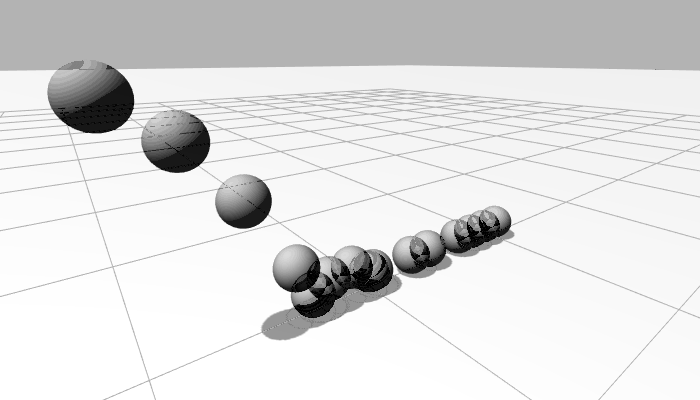
\includegraphics[width=0.8\textwidth]{images/contributions/chapter_7/bouncing_ball_trajectory.png}
    \caption{Sphere trajectory of the bouncing experiment.}
    \label{fig:bouncing_ball_trajectory}
\end{figure}

We consider a model composed of a single spherical-shaped link.
The sphere has a mass of $0.1 \, Kg$ and a radius of $10 \, cm$.
We approximate its collision shape with 500 points, all considered as collidable points for the collision detection and soft-contact model.

The sphere is positioned $1 \, m$ above a flat surface, and left falling starting from an initial linear velocity of $\vellin[B]_{W,B} = (2, 0, -1) \, m/s$.
We simulate this setting for $1.5 \, s$ using the \ac{RK4} integration scheme with a step size of $100 \, \mu s$.
The sphere's trajectory is illustrated in Figure~\ref{fig:bouncing_ball_trajectory}.

At each time instant, we compute the system's mechanical energy by summing the potential and the kinetic energies obtained from Equation~\eqref{eq:kinetic_and_potential_energies}.
We also get the linear contact forces $\forcelin[C_1]_1, \, \forcelin[C_2]_2, \, \dots$ computed with the soft-contact model of each collidable point, and combine them together in the frame $B$ of the spherical link as $\forcesix[B]_{tot} = \sum_i \transfor[B]^{C_i} \left[ \forcelin[C_i]_i^\top \;\; \zeros_3^\top \right]^\top \in \realn^6$.

Figure~\ref{fig:bouncing_ball} reports the height of the sphere corresponding to the $z$ component of $\pos[W]_B$, the plot of the mechanical energy, and the plot norm of the contact force's linear component.
It can be noticed that during the flight phase, the mechanical energy remains constant.
It gets dissipated abruptly through the contact damping upon bouncing collisions, and linearly through the terrain friction when bouncing finishes and the sphere starts rolling (corresponding to the flat region in Figure~\ref{fig:bouncing_ball_base_height}).
From the detailed view of the first two impacts reported in Figure~\ref{fig:bouncing_ball_detail1} and Figure~\ref{fig:bouncing_ball_detail2}, it can be noticed that the abrupt energy drop actually varies continuously.
From the same images, it can be seen that the soft-contact model produces contact forces that do not present marked discontinuities.
However, if the step size of the simulation becomes larger, we observed that the initial penetration depth could generate a big initial reaction force that depends on the stiffness of the terrain.
Possible solutions to mitigate this effect consists of either tuning the terrain parameters or adopting integration schemes with \emph{zero-crossing} logic that allow obtaining small initial penetration depths by shortening the integration step of the instant when the contact is made.

\begin{figure}
    \centering
    \subfloat[]{
        \includegraphics[width=0.95\textwidth]{images/contributions/chapter_7/bouncing_energy_force.tikz}
        \label{fig:bouncing_ball_complete}
    }
    \\
    \subfloat[]{
        \includegraphics[width=0.48\textwidth]{images/contributions/chapter_7/bouncing_energy_force_detail_1.tikz}
        \label{fig:bouncing_ball_detail1}
    }
    \subfloat[]{
        \includegraphics[width=0.42\textwidth]{images/contributions/chapter_7/bouncing_energy_force_detail_2.tikz}
        \label{fig:bouncing_ball_detail2}
    }
    \\
    \subfloat[]{
        \includegraphics[width=0.86\textwidth]{images/contributions/chapter_7/bouncing_base_height.tikz}
        \label{fig:bouncing_ball_base_height}
    }
    \caption{Evolution over time of the bouncing ball experiment's data. (\ref{fig:bouncing_ball_complete}) reports the mechanical energy of the system and the norm of the linear component of the contact forces summed and expressed in the $B$ frame of the spherical link. (\ref{fig:bouncing_ball_detail1}) and (\ref{fig:bouncing_ball_detail1}) report a closer view of the first two impacts. (\ref{fig:bouncing_ball_base_height}) reports the plot of the base height, where both the bouncing and rolling phases can be observed.}
    \label{fig:bouncing_ball}
\end{figure}

\subsection{Sliding Box on Flat Terrain}

We consider a model composed of a single box-shaped link.
The box has a mass of $1 \, Kg$ and $(x, y, z)$ dimensions equal to $(1.5, 1, 0.5) \, m$.
Its collision shape is approximated considering the 8 points corresponding to its corners.

The box is positioned on a flat ground surface at rest.
We simulate this setting for $4 \, s$ using the \ac{RK4} integration scheme with a step size of $1 \, ms$.
In this window, considering the frame of \ac{CoM} $G = (\pos[W]_{CoM}, [B])$, we apply to the \ac{CoM} of the box an external linear force $\forcelin[G]_{CoM} = (f_{CoM}, 0, 0) \in \realn^3$ with a profile reported in Figure~\ref{fig:sliding_box}.

In this setting, the threshold of the friction cone separating the sticking and the slipping regimes is $\mu f_\perp = 4.9 \, N$, averaged over the four contacts points of the bottom box surface.
Figure~\ref{fig:sliding_box} reports the plots of the $x$ components of the \ac{CoM}'s position and linear velocity.
It can be seen that, as expected, when the applied force is smaller than the threshold, the box stays still.
As soon as the external force exceeds the threshold, the box starts accelerating.
As soon as the external force goes to zero, the frictional effects of the contact model produce a reaction force that decelerates the box with a fast transient until it reaches the sticking regime again.
Small velocity oscillations can be noticed when the external force is applied at $t=0.5 \, s$ and $t=1 \, s$, and when it is removed at $t=3.5 \, s$.
They can be explained by the modelled dynamics of the material that can generate small tangential deformations without leaving the sticking regime.

\begin{figure}
    \centering
    \resizebox{0.75\textwidth}{!}{
    \includegraphics{images/contributions/chapter_7/sliding_box.tikz}}
    \caption{Evolution over time of the sliding box experiment's data. From top to bottom, the first plot shows the $x$ component of the \acs{CoM} position, the second plot shows the $x$ component of the \acs{CoM} velocity, and the third plot shows the profile of the applied external force to the \acs{CoM} frame $G$.}
    \label{fig:sliding_box}
\end{figure}

\subsection{Sliding Box on Inclined Plane}
\label{sec:sliding_box_inclined_plane}

\begin{figure}
    \centering
    \subfloat[]{
        \includegraphics{images/contributions/chapter_7/box_falling_inclined_mu_2.0}
        \label{fig:box_inclined_mu_2.0}
    }
    \\
    \subfloat[]{
        \includegraphics{images/contributions/chapter_7/box_falling_inclined_mu_0.0}
        \label{fig:box_inclined_mu_0.0}
    }
    \\
    \subfloat[]{
        \includegraphics{images/contributions/chapter_7/box_falling_inclined_mu_0.5}
        \label{fig:box_inclined_mu_0.5}
    }
    \caption{Comparison of the box's \acs{CoM} trajectory simulated with the proposed soft-contact model and the Mujoco simulator, considering a coefficient of friction (a) $\mu=2$, (b) $\mu=0$, (c) $\mu=0.5$.}
    \label{fig:box_inclined_mu}
\end{figure}

We consider a model composed of a single box-shaped link.
The box has a mass of $1 \, Kg$ and $(x, y, z)$ dimensions equal to $(0.15, 0.1, 0.05) \, m$.
Its collision shape is approximated considering the 8 points corresponding to its corners.

\begin{table}
\small
\centering
\caption{Mujoco configuration considered in the experiments of the sliding box on inclined surface matching as close as possible the setting and properties of our soft-contact model. Refer to the official documentation at \url{https://mujoco.readthedocs.io} for a detailed explanation of the options.}
\label{tab:mujoco_parameters}
\begin{tblr}{
    colspec={Q[c, m]Q[c, m]},
    row{even} = {bg=gray9},
    row{1} = {font=\bfseries\footnotesize},
}
    \toprule
    Property & Value \\
    \midrule
    \texttt{timestep} & $0.001$ \\
    \texttt{integrator} & \texttt{RK4} \\
    \texttt{solver} & \texttt{Newton} \\
    \texttt{iterations} & $50$ \\
    \texttt{cone} & \texttt{elliptic} \\
    \texttt{friction} & $(\mu,\, 0,\, 0)$ \\
    \texttt{solref} & $(-1e6,\, -2000)$ \\
    \texttt{condim} & $3$ \\
    \bottomrule
\end{tblr}
\end{table}

The box starts floating in the air having its \ac{CoM} positioned in $\pos[W]_G = (0, 0, 1.0) \, m$.
Then, we let the box fall due to gravity over a plane inclined by $20\degree$ so that the box slides down in the direction of the $x$ axis.
In this setting, we perform three experiment each characterised by a different coefficient of friction $\mu$.
We simulate this setting for $2.5 \, s$ using the \ac{RK4} integration scheme with a step size of $1 \, ms$.
For validation purpose, we simulate the same setting with the Mujoco simulator configured with comparable physics parameters, reported in Table~\ref{tab:mujoco_parameters}.
In particular, Mujoco provides a similar spring-damper soft-contact model that we can consider as ground truth.

In the first experiment, we consider an extremely large $\mu = 2.0$ so that we can assess how the selected stiffness $k$ and damping $\lambda$ affect the landing over the inclined plane without accounting for major sliding effects.
From Figure~\ref{fig:box_inclined_mu_2.0}, it can be noticed that the falling trajectories due to gravity overlap perfectly until the impact.
After the impact, the $y$ position of both boxes always remains constant, showing that in both cases the generated tangential forces do not have any $y$ component.
In our soft-contact model this means that no material deformation occurs in this direction, as expected.
The $x$ and $z$ components, although not matching perfectly due to the different formulation of the soft contacts --mainly due to Equation~\eqref{eq:soft_contact_normal_force}-- are sufficiently close and show the same qualitative behaviour.

In the second experiment, we consider a friction-less simulation with $\mu = 0$.
In this setting, our soft-contact model only produces normal forces proportional to the penetration depth.
The friction cone cannot be evaluated and no tangential forces are produced, therefore the only possible regime is sliding.
Figure~\ref{fig:box_inclined_mu_0.0} reports the trajectories of the two falling boxes, showing in this case almost a perfect match between our soft-contacts model and Mujoco.

In the third experiment, we consider a realistic coefficient of friction $\mu = 0.5$.
The combination of this coefficient of friction with the inclination of the terrain has been selected for reaching a steady sticking regime after an initial sliding regime right after the impact.
Figure~\ref{fig:box_inclined_mu_0.5} shows the trajectories of the two boxes.
Also in this case, after the impact, both simulations correctly do not produce tangential forces in the $y$ direction.
The $x$ and $z$ components, similarly to the $\mu = 2.0$ case, do not match perfectly but also in this case show the same qualitative behaviour where the box transitions from the sliding to a steady sticking regime approximately at $t=1.2~s$.

All three experiments show that the proposed contact model behaves similarly to the ground truth represented by the soft-contact model implemented in the Mujoco simulator.
The qualitative behaviour always look alike, although the trajectories do not necessarily match quantitatively.
The main reason for the numerical mismatch is twofold.
First, the formulation used to compute the normal force differs from Equation~\eqref{eq:soft_contact_normal_force}.
This difference propagates also to the tangential component since the sticking-slipping boundary is a function of the normal force.
Furthermore, the methodology to compute the contact force is completely different.
In fact, we use a continuous contact model that introduces an additional state to the \ac{ODE} describing the dynamics of the multi-body system.
Mujoco, instead, at each time step solves a constrained quadratic optimisation problem.
Further details on the internal details of Mujoco contacts can be found in \parencite{todorov_convex_2014, vousten_simulating_2022, yoon_comparative_2023}.

\newpage
\section{Conclusions}

In this chapter, we described how to model a floating-base multibody system interacting with a non-flat surface.
This formulation lays the fundamentals of a physics engine, capable of simulating the evolution of such systems in time.
We introduced a point-surface soft-contact model to compute the forces exchanged between points belonging to the links of the multibody system and a non-flat terrain, assuming to know its height profile at any point in space.
This assumption simplifies the collision detection process, requiring just trivial geometrical assessments.
The main benefit of our collisions and contacts modelling is the possibility of obtaining an extended state-space representation that includes both the dynamics of the multibody system and the dynamics of the contacts.
The contact-aware evolution of the system can be derived by any numerical integration scheme.
We validated the dynamical system in two simplified settings.
In the first one, we considered single bodies interacting with a flat terrain, showing the continuity of the soft-contacts model and the switching between the sticking and slipping regimes.
In the second one, we considered non-flat terrain, showing the trajectory of a box falling over an inclined plane characterised by different coefficients of friction.
While sphere and box collisions might seem trivial examples, they often represent the typical collision shapes adopted to simulate robot's feet.

The final contact-aware dynamical system combined with the point-surface collision detection logic presents different limitations, especially when compared to implementations provided by general-purpose simulators.
Our solution does not support detecting collisions between different bodies and does not consider joint limits and other types of constraints.
To address the former, more advanced geometrical processing is necessary for detecting all ranges of collisions between points, primitive shapes, edges, surfaces, \etc
For the latter, instead, it is possible to introduce an additional phase in the simulation step that computes the generalized forces to apply to the system for enforcing those constraints.
